\documentclass[../thesis]{subfiles}

\begin{document}
	\section{Heterogeneous Platforms}
	\label{sec:techbg:hetplats}

	As the evolution of microprocessors moves towards higher levels of parallelism, several other options exist, from using multiple machines in a cluster, allowing each to perform part of the computation independently, to specific-purpose devices such as \dsps and \gpus.

	\begin{wrapfigure}{r}{0.4\textwidth}
		\centering
		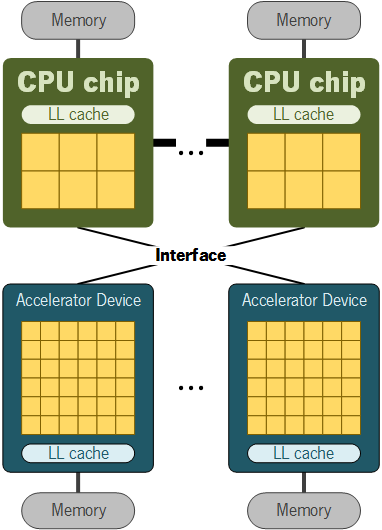
\includegraphics[width=0.35\textwidth]{assets/images/techbg/hetplat.png}
		\captionsetup{font=small}
		\caption{Example of a computing node architecture.}
		\label{fig:cudacore}
	\end{wrapfigure}

	\tdg{definition of hetplats}%
	A given system is said to be heterogeneous when it contains multiple devices of different kinds. Usually, each of these devices is capable of computing several operations in parallel. The most efficient computing systems of the world in the TOP500 list\footnote{\url{http://www.top500.org}} are composed of several interconnected computing nodes, each with multiple multicore \cpus and one or more specialized hardware accelerators. \gpus and \intel\xeon Phi coprocessors are currently the most popular.

	\tdg{GPUs and MICs (summary)}%
	Popularity of these new specialized devices in \hpc, some created and developed in completely separate environments, has been increasing in the last years, triggered by the trend to use the number of cores in computing hardware. \gpus evolution, for example, where execution throughput is more important than execution latency, led to massively parallel architectures, able to process hundreds of pixels at the same time. Devices based on the \intel\mic architecture, on the other hand, are placed between \gpus and \cpus, having the characteristics for massive parallelism while still being able to handle more complex operations (such as running an operating system). Both kinds of devices are explained in more depth in \cref{chp:cuda,chp:mic} where they are explored in the context of this document's case study.

	\tdg{alternative accelerators}%
	\dsps are another class of accelerators recently made popular for \hpc due to new architectures able to perform floating-point computations. Their architecture is very similar to that of a conventional processor, both programming and memory-wise \cite{FLAWN61}. Alternatively, \fpgas mix a set of configurable logic blocks, digital signal processor blocks and traditional \cpu cores (optional), all using a configurable interconnect. The key characteristic of these devices is the ability to configure them for a specific type of computation making them extremely versatile \cite{Brodtkorb:2010}. These devices are described here for completeness, not being the scope of this document to explore the case study using them.

	\tdg{processor-memory gap in accelerators}%
	Most computing accelerators suffer from the same limitations as conventional processor architectures regarding memory latency (explained in \cref{sec:techbg:distmem}), despite the many strategies each one implements to hide or overcome the problem. Also, since the connection between the \cpu and an accelerator is typically performed over a \pcie interface, using the same memory banks would be a major bottleneck. For this reason, most devices have their own built-in memory hierarchy, which is managed in a space distinct of the \cpus.
\end{document}
